%!TEX root = ../../presentation.tex

\begin{frame}{The Embedded Finite Element Method - Continuum Setting}

\begin{reference}{\refh}{\refv}
Simo et al. (1993), Armero (1999), ...
\end{reference}


\vspace*{-3mm}

\begin{figure}
\centering
{\footnotesize
  \psfrag{O}[c][c]{\parbox{3cm}{\centering{global continuum\\ mechanical BVP}}}
  \psfrag{M}[c][c]{\parbox{3cm}{\centering{local mechanical\\ continuum problem}}}
  \psfrag{N}[c][c]{\parbox{3cm}{\centering{local electrical\\ continuum problem}}}
  \psfrag{B}[c][c]{$\body$}
  \psfrag{U}[c][c]{$\partial_u\body$}
  \psfrag{T}[l][l]{$\partial_t\body$}
  \psfrag{F}[c][c]{$\partial_\emP\body$}
  \psfrag{Q}[c][c]{$\partial_\emsurfcharge\body$}
  \psfrag{X}[c][c]{$\body_x$}
  \psfrag{G}[c][c]{\red{$\Gamma_x$}}
  \psfrag{b}[c][c]{$\rho\Bb$}
  \psfrag{x}[c][c]{$\Bx$}
  \psfrag{m}[c][c]{$\Bn$}
  \psfrag{t}[c][c]{$\bar\Bt$}
  \psfrag{n}[c][c]{$\Bn$}
  \psfrag{w}[c][c]{$\bar\emsurfcharge$}
  \psfrag{q}[c][c]{$\emfreecharge$}
  \psfrag{j}[c][c]{\red{$\jump{\Bu}$}}
  \psfrag{k}[c][c]{\red{$\jump{\emP}$}}
  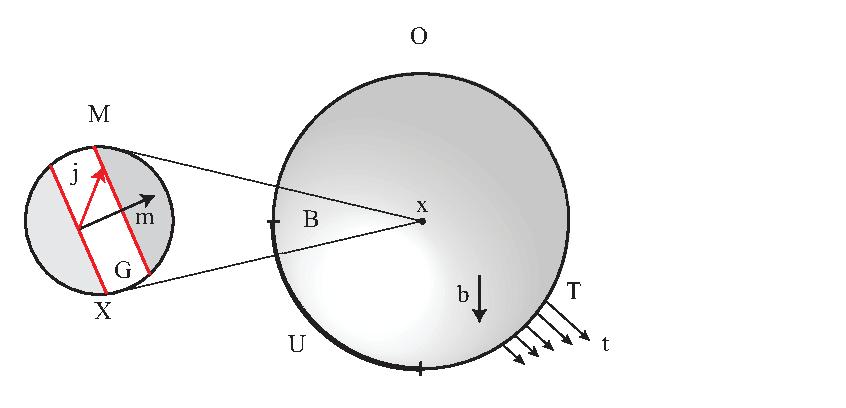
\includegraphics[height=35mm]{\slidedir/f01.eps}
}
\end{figure}

\bigskip

Decomposition of the displacement field into a global and a discontinuous part:
\begin{equation*}
\Bu_\mu=\Bu+\tilde\Bu(\jump{\Bu_\mu})\quad\text{in}\quad\body_x
\end{equation*}

\smallskip

Decomposition of the strain field into a global and a discontinuous part:
\begin{equation*}
\Bvarepsilon_\mu=\Bvarepsilon+\tilde\Bvarepsilon(\jump{\Bu_\mu})\quad\text{in}\quad\body_x\backslash\Gamma_x
\end{equation*}

\smallskip

Incorporation of displacement jumps $\jump{\Bu_\mu}$ into the weak equations:
\begin{equation*}
\int_{\body}\Bsigma:\nabla^s\delta\Bu\dV=
\int_{\body}\rho\Bb\cdot\delta\Bu\dV+
\int_{\partial_t\body}\bar\Bt\cdot\delta\Bu\dA
\AND
\int_{\Gamma_x}\delta\jump{\Bu_\mu}\cdot(\Bsigma\Bn-\Bt_\Gamma)\dA=0
\end{equation*}

\smallskip

\end{frame}
